\documentclass[a4paper, 12pt]{article}

\usepackage{bera}% optional: just to have a nice mono-spaced font
\usepackage{listings}
\usepackage{xcolor}
\usepackage{tikz}

\usepackage{listings}
\usepackage{color}
\usepackage{booktabs, makecell, colortbl}

\definecolor{dkgreen}{rgb}{0,0.6,0}
\definecolor{gray}{rgb}{0.5,0.5,0.5}
\definecolor{mauve}{rgb}{0.58,0,0.82}
\definecolor{gray}{rgb}{0.4,0.4,0.4}
\definecolor{darkblue}{rgb}{0.0,0.0,0.6}
\definecolor{lightblue}{rgb}{0.0,0.0,0.9}
\definecolor{cyan}{rgb}{0.0,0.6,0.6}
\definecolor{darkred}{rgb}{0.6,0.0,0.0}


\colorlet{punct}{red!60!black}
\definecolor{background}{HTML}{EEEEEE}
\definecolor{delim}{RGB}{20,105,176}
\colorlet{numb}{magenta!60!black}

\lstdefinelanguage{json}{
    basicstyle=\normalfont\ttfamily,
    numbers=left,
    numberstyle=\scriptsize,
    stepnumber=1,
    numbersep=8pt,
    showstringspaces=false,
    breaklines=true,
    frame=lines,
    backgroundcolor=\color{background},
    literate=
     *{0}{{{\color{numb}0}}}{1}
      {1}{{{\color{numb}1}}}{1}
      {2}{{{\color{numb}2}}}{1}
      {3}{{{\color{numb}3}}}{1}
      {4}{{{\color{numb}4}}}{1}
      {5}{{{\color{numb}5}}}{1}
      {6}{{{\color{numb}6}}}{1}
      {7}{{{\color{numb}7}}}{1}
      {8}{{{\color{numb}8}}}{1}
      {9}{{{\color{numb}9}}}{1}
      {:}{{{\color{punct}{:}}}}{1}
      {,}{{{\color{punct}{,}}}}{1}
      {\{}{{{\color{delim}{\{}}}}{1}
      {\}}{{{\color{delim}{\}}}}}{1}
      {[}{{{\color{delim}{[}}}}{1}
      {]}{{{\color{delim}{]}}}}{1},
}

\lstset{
  basicstyle=\ttfamily\footnotesize,
  columns=fullflexible,
  showstringspaces=false,
  numbers=left,                   % where to put the line-numbers
  numberstyle=\tiny\color{gray},  % the style that is used for the line-numbers
  stepnumber=1,
  numbersep=5pt,                  % how far the line-numbers are from the code
  backgroundcolor=\color{white},      % choose the background color. You must add \usepackage{color}
  showspaces=false,               % show spaces adding particular underscores
  showstringspaces=false,         % underline spaces within strings
  showtabs=false,                 % show tabs within strings adding particular underscores
  frame=none,                   % adds a frame around the code
  rulecolor=\color{black},        % if not set, the frame-color may be changed on line-breaks within not-black text (e.g. commens (green here))
  tabsize=2,                      % sets default tabsize to 2 spaces
  captionpos=b,                   % sets the caption-position to bottom
  breaklines=true,                % sets automatic line breaking
  breakatwhitespace=false,        % sets if automatic breaks should only happen at whitespace
  title=\lstname,                   % show the filename of files included with \lstinputlisting;
                                  % also try caption instead of title  
  commentstyle=\color{gray}\upshape
}


\lstdefinelanguage{XML}
{
  morestring=[s][\color{mauve}]{"}{"},
  morestring=[s][\color{black}]{>}{<},
  morecomment=[s]{<?}{?>},
  morecomment=[s][\color{dkgreen}]{<!--}{-->},
  stringstyle=\color{black},
  identifierstyle=\color{lightblue},
  keywordstyle=\color{red},
  morekeywords={xmlns,xsi,noNamespaceSchemaLocation,type,id,x,y,source,target,version,tool,transRef,roleRef,objective,eventually}% list your attributes here
}

\usepackage[utf8]{inputenc}
\usepackage[T1]{fontenc}
\usepackage[french]{babel}
\usepackage{graphicx}
\usepackage{amsmath}
\usepackage{hyperref}
\usepackage{lmodern}
\usepackage{moreverb}
\usepackage{multicol}
% Please add the following required packages to your document preamble:
 \usepackage[table,xcdraw]{xcolor}
% If you use beamer only pass "xcolor=table" option, i.e. \documentclass[xcolor=table]{beamer}
 \usepackage[normalem]{ulem}
\useunder{\uline}{\ul}{}



\usepackage[a4paper,left=2cm,right=2cm,top=2cm,bottom=2cm]{geometry}

\pagestyle{headings}
\pagestyle{plain}


\setcounter{secnumdepth}{4}
\setcounter{tocdepth}{4}
\makeatletter


\makeatother



\makeatletter
\def\toclevel@subsubsubsection{4}
\def\toclevel@paragraph{5}
\def\toclevel@subparagraph{6}
\makeatother


\setlength{\parindent}{0cm}
\setlength{\parskip}{1ex plus 0.5ex minus 0.2ex}
\newcommand{\hsp}{\hspace{20pt}}
\newcommand{\HRule}{\rule{\linewidth}{0.5mm}}



\begin{document}

\begin{titlepage}
  \begin{sffamily}
  \begin{center}

   
  \textsc{\LARGE }\\[2cm]

    \textsc{\Large Document de définition de l’application}

    % Title
    \HRule \\[0.4cm]
    { \huge  \textsc{Projet d'interopérabilité} \\
    \textsc{\small Groupe 4}\\ [0.4cm] }
	

    \HRule \\[2cm]
    \textsc {Idriss BENGUEZZOU\\ Iness BOUABID\\Ali BOUGASSAA\\Ghilas MEZIANE }
 \begin{figure}
     \centering
    
\includegraphics[scale=0.2]{logoUJM.png}
     \label{fig:ujm_logo}
 \end{figure}
   
    \

    \vfill

    % Bottom of the page
    {\large {} 08/02/2023}

  \end{center}
  \end{sffamily}
\end{titlepage}


\newpage
\tableofcontents

\newpage
\section{Objet du document}

L'objectif de ce document de définition de l'application est de fournir une description détaillée de l'application, en mettant l'accent sur trois aspects clés : l'usage ciblé, l'environnement Wikibase et l'exploitation.

La première partie de ce document se concentrera sur l'usage ciblé de l'application. Elle fournira une description de l'utilisation prévue de l'application, en identifiant les objectifs et les besoins des utilisateurs finaux.

La deuxième partie de ce document sera consacrée à l'environnement Wikibase. Elle fournira une description détaillée de l'environnement dans lequel l'application sera déployée, en mettant l'accent sur les exigences techniques et les contraintes.

La troisième partie de ce document se concentrera sur l'exploitation de l'application. Elle fournira des informations sur la maintenance, la surveillance et la gestion de l'application une fois qu'elle est déployée. Cette section expliquera également comment l'application sera supportée, maintenue et améliorée au fil du temps pour garantir qu'elle reste efficace et fiable.


\section{Usage ciblé}

Le projet WikibaseLocale vise à promouvoir la vie culturelle et à améliorer la connaissance des lieux culturels dans la région en créant une base de données centralisée vivante. Les futurs acteurs et utilisateurs de cette base sont les citoyens, les entreprises, les collectivités locales, les écoles, les bibliothèques, les associations, l'office du tourisme, etc.

L'objectif de WikibaseLocale est de fournir un outil de recherche centralisé pour permettre aux utilisateurs de trouver des informations sur les lieux culturels tels que les théâtres, les musées et les galeries d'art, ainsi que leurs expositions et événements à venir. Les utilisateurs peuvent effectuer des recherches simples ou plus avancées pour trouver des informations sur les lieux culturels dans leur ville ou quartier.

En résumé, l'usage ciblé de WikibaseLocale est de fournir une base de données centralisée pour la recherche d'informations sur les lieux culturels, afin de promouvoir la vie culturelle et la connaissance des lieux dans la région.

\section{Environnement Wikibase}

WikibaseLocale sera développé dans l'environnement Wikibase, qui est une plateforme open-source de gestion de données qui permet de stocker, d'éditer et de publier des données structurées.

La base de données de WikibaseLocale sera constituée de données hétérogènes et diverses sur les lieux culturels, y compris des informations sur les théâtres, les musées et les galeries d'art, leurs adresses, leurs expositions et événements à venir.

Pour alimenter la base de données de WikibaseLocale, il faudra collecter des données de différentes sources et les structurer.

\section{Exploitation}

Une fois que la base de données de WikibaseLocale est constituée, elle sera maintenue pour assurer sa pertinence et sa qualité. Les données seront régulièrement mises à jour pour refléter les changements dans les lieux culturels et les événements à venir.

Pour faciliter l'accès aux informations sur les lieux culturels, une web application sera mise en place. Cette application offrira une expérience utilisateur ergonomique pour effectuer des recherches simples ou avancées. Les utilisateurs pourront filtrer les résultats de recherche en fonction de leur emplacement et de leurs centres d'intérêt.

L'application sera accessible en ligne via un navigateur Web, ce qui permettra aux utilisateurs d'y accéder facilement à partir de leur ordinateur, tablette ou smartphone. Elle sera également compatible avec les différents navigateurs Web couramment utilisés, afin de garantir une expérience utilisateur optimale.

Pour pouvoir exploiter ces données nous metterons en place deux application. Une première dédié à l'injection et la mise à jour des données dans notre wikibase, et une seconde permettant de questionner notre wikibase depuis une interface web.

Ci-dessous, un schéma représentant les interactions de premier niveau du système wikistone.

\begin{figure}[h]
    \centering
    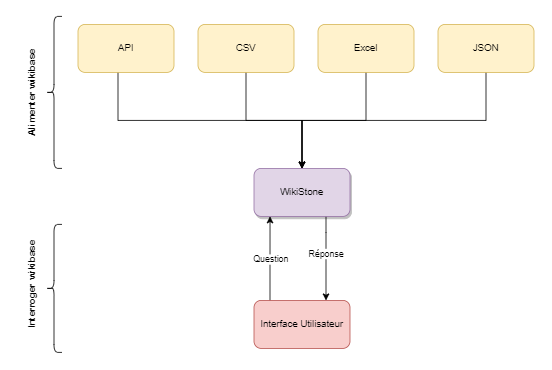
\includegraphics[scale=0.75]{schema-general.png}
    \caption{Représentation générale}
    \label{fig:my_label}
\end{figure}

\end{document}